\section{Copyright-Protecting Model Fusion}

We focus on language models \( p \) that take a prompt \( x \) as input and return a probability distribution over a sequence of tokens of variable length \( T \) from a fixed alphabet \( V \), with \( y_T = \text{EOS} \) representing the end-of-sequence token.  Using
the convention that  \( y_{<0} = \emptyset \), we can factorize $p$ as:
$$
p(y_{0:T} | x) = \prod_{t=0}^T p(y_t | y_{<t}, x).$$
We now introduce a key assumption and background underlying our work.


\subsection{Preliminaries}
\label{sec:preliminaries}
At the core of our method is the assumption of the \textit{separability of copyrighted material}, as discussed by \citet{vyas2023provable} for various vision and language applications. This assumption is akin to those used in exact machine unlearning \citep{bourtoule2021machine,yan2022arcane, dukler2023safe} and in works that split datasets into safe and unsafe parts \citep{golatkar2021mixed, golatkar2024cpr, li2024purifying}.

Consider a dataset $\dataset$ and a set of copyright-protected material $\domainconcepts$ that could be compromised when training a model $\model$ on $\dataset$. The assumption states that we can split $\dataset$ into two potentially overlapping subsets, $\dataset_1$ and $\dataset_2$, such that each subset contains data associated with two non-overlapping sets of copyright-protected materials, $\domainconcepts_1$ and $\domainconcepts_2$, where $\domainconcepts_1 \cap \domainconcepts_2 = \emptyset$. This assumption holds, for instance, when we construct $\dataset$ from sources that are sufficiently distinct. Hence, any language model trained on the subset $\dataset_1$ is protected from infringing the copyright of materials in $\domainconcepts \setminus \domainconcepts_1 \supseteq \domainconcepts_2$.

Given the two subsets $\dataset_1$ and $\dataset_2$, we can then train two generative models $p^{(1)}$, $p^{(2)}$ on the respective subsets and ``fuse'' them to construct a model $p$ that achieves protection against all copyright-protected material $\mathcal{C}$. In this context, \citet{vyas2023provable} propose the $k$-NAF (Near Access Free) framework as a quantitative guarantee for copyright protection. 
\begin{definition}
\label{def:knaf}
Formally, a model $ p(. | x)$ is $k$-NAF for some $k\in \RR^+$ if, for any input prompt $x$ and some user-specified divergence function~$\Delta$,
\begin{equation}\label{eq:minkl}
  \forall x: \quad  \max_{i \in \{1,2\}} \Delta( p(. | x) \mid\mid p^{(i)}(. | x)) \leq k.
\end{equation}
\end{definition}
The key intuition behind why a model satisfying $k$-NAF is less likely to regurgitate copyrighted material is as follows: if the separability of copyrighted material holds, the likelihood of generating infringing text for any material $c \in \domainconcepts$ decreases exponentially with the length of $c$ for at least one of the models. Therefore, for a model $p$ to satisfy the $k$-NAF guarantee, it must assign a minimal probability to events involving the reproduction of protected material.


% In the following section, 

\subsection{Algorithm}
\label{sec:algo}

We introduce \textbf{C}opyright-\textbf{P}rotecting Model \textbf{Fus}ion (CP-Fuse), a simple yet effective algorithm for copyright protection via model fusion. Inspired by the $k$-NAF framework, we aim to minimize the maximum KL-divergence in Equation~\eqref{eq:minkl}. However, achieving this directly is computationally intractable; therefore, we propose an efficient approximate algorithm that iteratively optimizes $p(y_{t} | y_{<t}, x )$ given the probability of the history $p(y_{<t} | x )$. In Lemma~\ref{lem:kkt}, we show that leveraging the KL-divergence allows us to express the update rule in a model fusion form. Formally, we iteratively define
 %\fy{the minimizer should be pstar (if consistent with intro e.g.) and argument p? - not consistent throughout the section - 2. also in the next equation, p is not defined? 3. do we even need to compute the term after KL? isn't the minmization just over the KL term and its done? (like in the teaser figure)}
\begin{equation}
\label{eq:pt}
    \begin{aligned}
        p(y_t \, | \, y_{<t}, x) &= \arg\min_{p^*} \max_i \underset{y_t \sim p^*}{\mathbb{E}} \log\left( \frac{p^*(y_t) p(y_{<t} \, | \, x)}{\modeli(y_{\leq t} \, | \, x)} \right)\\
            &=\arg\min_{p^* , t} ~t \quad \text{s.t.}~~\\ \forall i: ~~ \text{KL}( p^*\vert &\vert p^{(i)}(. \vert y_{<t}, x) ) + \log\left(\frac{p(y_{<t} \, | \, x)}{\modeli(y_{< t} \, | \, x)} \right) \leq t,
    \end{aligned}
\end{equation}
which results in a convex optimization problem. Although solving this problem naively is still computationally intensive, we overcome this limitation using the following lemma:
\begin{lemma}
\label{lem:kkt}
The optimal solution \(  p(y_t \, | \, y_{<t}, x)\) of the optimization problem in Equation~\eqref{eq:pt} satisfies\footnote{We set \(\log(0) = - \infty\)}
\begin{equation}
    \begin{aligned}
    \log p^*(y_t) &= \alpha_t \log \modelone(y_t | y_{<t}, x)  + \beta_t \log \modeltwo(y_t | y_{<t}, x) + \gamma_t
    \end{aligned}
\label{eq:opt}
\end{equation}
for some \(\alpha_t, \beta_t \geq 0, \gamma_t \in \mathbb{R}\).
\end{lemma}
Equation~\eqref{eq:pt} can therefore be solved efficiently by performing a grid search over the parameters \(\alpha_t\) and \(\beta_t\), with \(\gamma_t\) chosen as a function of \(\alpha_t\) and \(\beta_t\) to ensure the total probability mass sums to 1.


\paragraph{Related works on model fusion}
Our method is reminiscent of an extensive body of work focused on knowledge fusion in language models, both at inference time \citep{liu2021dexperts, jiang2023llm, gururangan2023scaling, mavromatis2024pack} and through weight merging after training \citep{wortsman2022model, jin2022dataless, hsu2024let, yadav2024ties}. In particular, the minimizer derived in \Cref{lem:kkt} relates to the former approaches, which generally define a model $p$ at inference time by combining multiple models $p^{(1)}, \dots, p^{(K)}$ via a weighted sum of their logits:
\begin{equation}
\label{eq:fusion}
\log p(y_t | y_{<t}, x) := 
    \sum_{i=1}^K \alpha_t^{(i)}(y_{<t}, x) \log p^{(i)}(. | y_{<t}, x) + c,
\end{equation}
where $c$ is a normalizing constant, and $\alpha_t^{(i)}$ can depend on both the prompt $x$ and the history $y_{<t}$. However, previous model fusion approaches are not designed to mitigate copyright infringement.


\citet{vyas2023provable} propose $\cpdelta$ as a general strategy for combining two generative models aimed at achieving copyright protection. Yet, their approach becomes computationally intractable when applied directly to the probability distribution \( p(.| x) \) over the entire sequence \( y_T \). To address this, the authors suggest applying $\cpdelta$ token-wise instead, resulting in the model from \Cref{eq:opt} with $\alpha_t = \beta_t = 1/2$. However, they do not benchmark this method against other copyright-protection techniques. In the following section, we discuss why this approach is ineffective for copyright protection and how our method overcomes this issue by incorporating the sequence history \( y_{<t} \).




% do not enforce $p$ to be close to all models $p^{(i)}$ simultaneously. 
% Independently, token-wise $\cpdelta$ has also been used in a slightly different context for purifying language models \citep{li2024purifying}


\subsection{Efficacy of methodology}
In this section, we provide an intuitive explanation of how our method prevents the reproduction of memorized training samples.  Recall that, by \Cref{lem:kkt}, CP-Fuse adaptively selects $\alpha_t$ and $\beta_t$ based on the sequence history $y_{<t}$. Specifically, the algorithm assigns less weight to the model that has been more dominant in generating $y_{<t}$. More formally, the following balancing property holds:

\begin{lemma}
\label{lem:balance}
(Balancing property) Given a prompt $x$, let \( y_{<t} \) be any non-ending sequence and assume that $p^{(i)}(. \vert y_{<t} , x) $ has full support for $i\in \{1,2\}$ and  \( p^{(1)}(y_{<t} | x) > \modeltwo(y_{<t} | x) \). Then, either
%either \fy{exactly one or at least one?} of the two cases is true:
\begin{align*}
    1. &  \underset{y_{t} \sim p(. | y_{<t}, x)}{\mathbb{E}} \log \modelone(y_{\leq t} \vert x)  \quad =  \underset{y_{t} \sim p(. | y_{<t},x)}{\mathbb{E}} \log \modeltwo(y_{\leq t} \vert x) \\
    2. &  \quad \quad \quad \quad \quad p(y_t | y_{<t}, x)  = \modeltwo(y_t | y_{<t}, x) 
\end{align*}
\end{lemma}



\begin{wrapfigure}{r}{0.50\textwidth}
\vspace{-0.4cm}
    \centering
    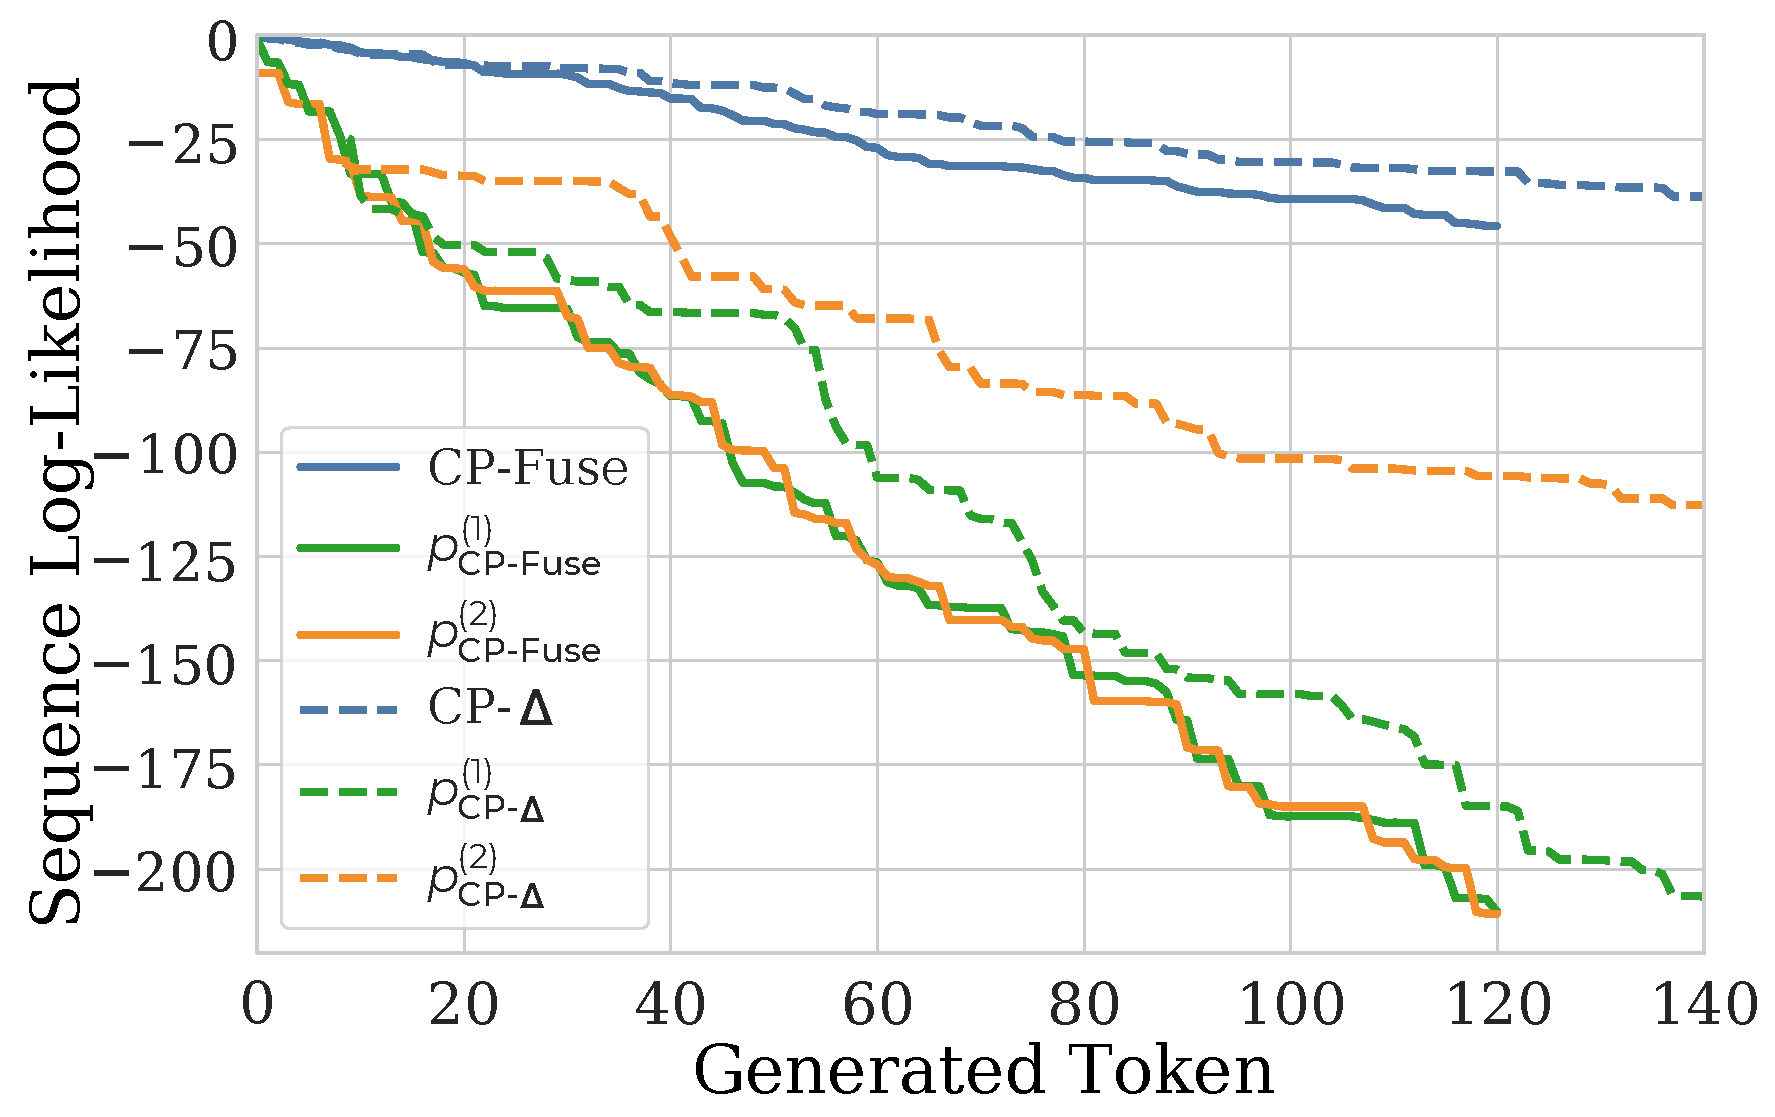
\includegraphics[width=0.50\textwidth]{figures/cumulative_combined.pdf}
    \caption{Log-likelihood of sequences produced by CP-Fuse and $\cpdelta$, and their base models $p^{(1)}$ and $p^{(2)}$, at each generated token. We show a random generation from StarCoder fine-tuned on the \texttt{Python instructions}; details in \Cref{sec:experiments}. }
    \label{fig:cumulative_main}
     \vspace{-0.4cm}

\end{wrapfigure}

Intuitively, this balancing property ensures that neither model dominates the text generation. As an example, suppose the generation of a subsequence \( y_{<t} \) is strongly dominated by $\modelone$, such that \( \modelone(y_{<t} | x) \gg \modeltwo(y_{<t} | x) \). If the first case in \Cref{lem:balance} holds, the output distribution of the copyright-protected model, \( p(y_t | y_{<t}, x) \), will be such that, in expectation,  the sequence with the new token has the same log-probability for both models, i.e., loosely speaking $\modelone(y_{\leq t} | x) \approx \modeltwo(y_{\leq t} | x)$.
%much closer to \fy{here you mean yt | y<t... conditional} \( \modeltwo(y_{<t} | x) \) than to \( \modelone(y_{<t} | x) \).
Conversely, if the second case \( p = \modeltwo \) holds, then the generation of \( y_t \) is independent of \( \modelone(y_{<t} | x) \). In other words, the next token generated by \( p \) will likely match the most probable token under the dominant model, \( \modelone(y_{<t} | x) \), only if both \( \modelone \) and \( \modeltwo \) are close conditioned on \( y_{<t} \) and \( x \), that is, when the generated sequence is not protected assuming separability of copyrighted material (\Cref{sec:preliminaries}). 
We provide additional experimental evidence for this property in \Cref{app:weights}.
% \fy{I'd rather say: If one model is dominant for some token, then p will assign much smaller probability to that token.}




% \begin{wrapfigure}{r}{0.46\textwidth}
% \vspace{-0.4cm}
%     \centering
%     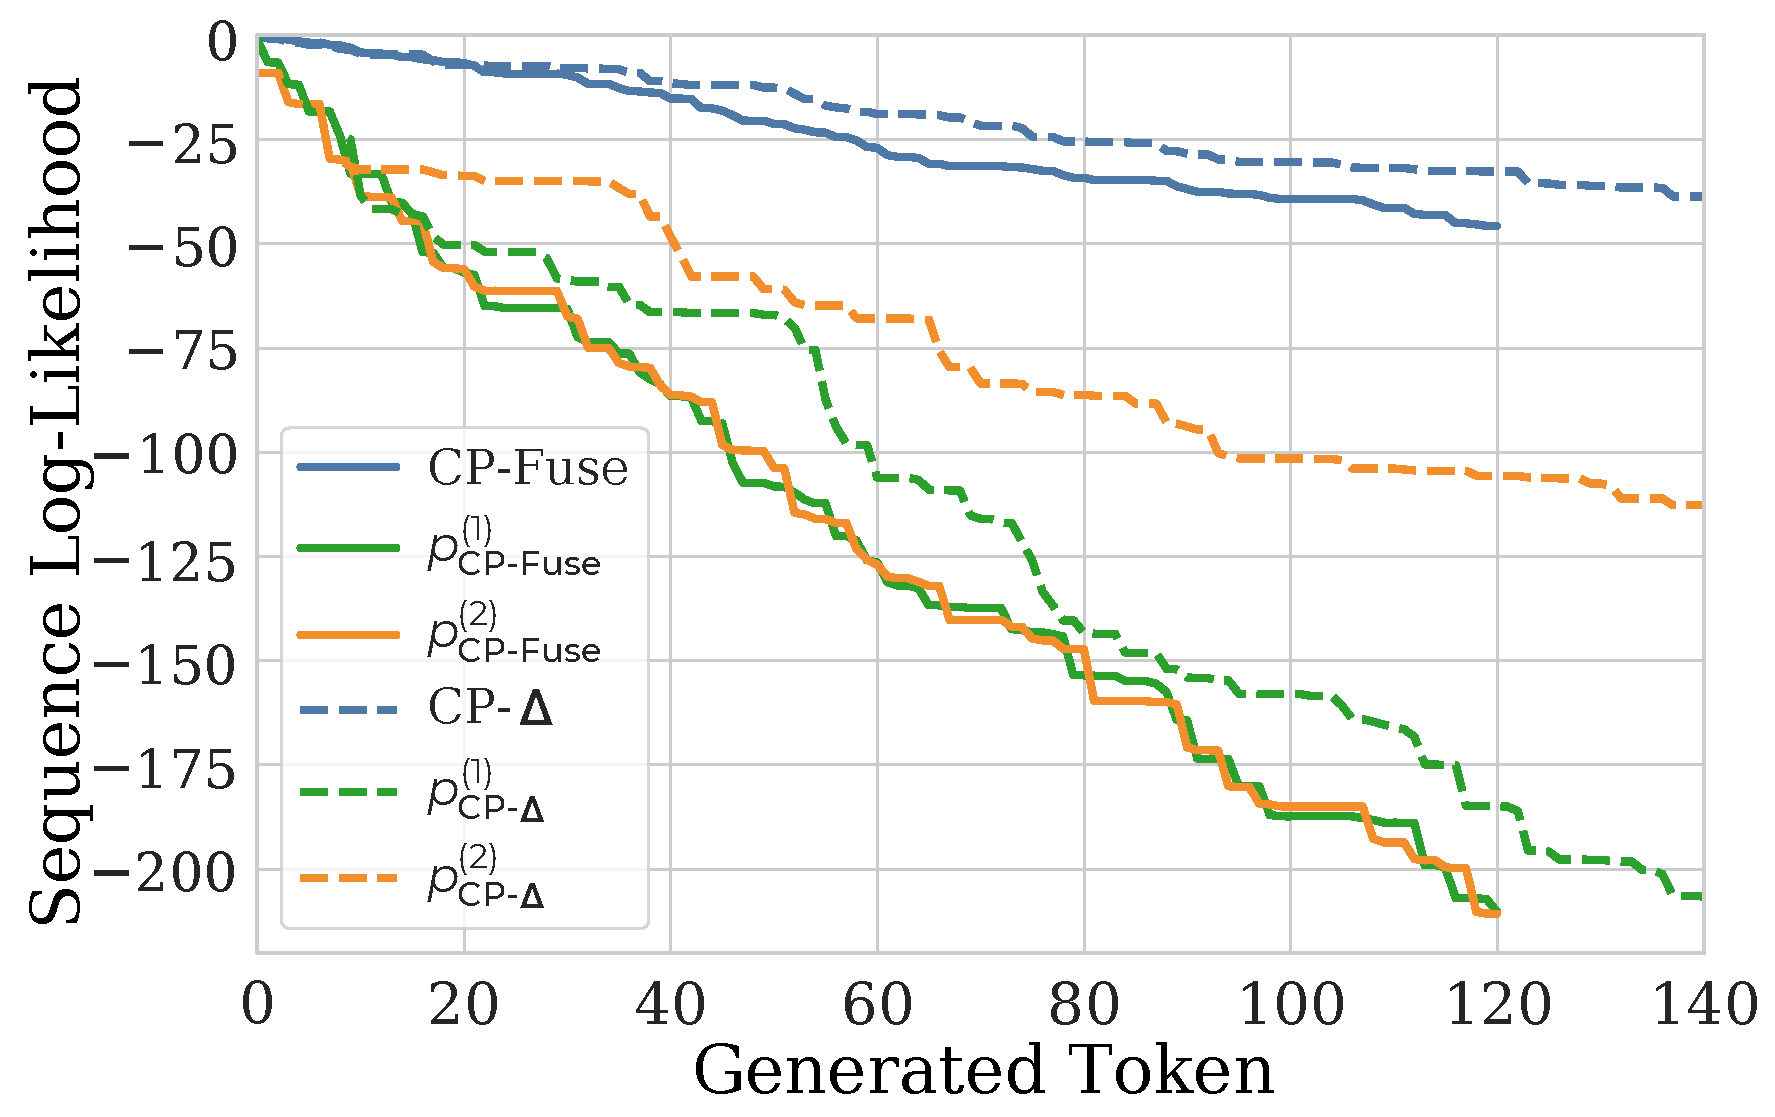
\includegraphics[width=0.46\textwidth]{figures/cumulative_combined.pdf}
%     \caption{Log-likelihood of sequences produced by CP-Fuse and $\cpdelta$, and their base models $p^{(1)}$ and $p^{(2)}$, at each generated token. We show a random generation from StarCoder fine-tuned on the \texttt{Python instructions}; details in \Cref{sec:experiments}. }
%     \label{fig:cumulative_main}
%      \vspace{-0.5cm}

% \end{wrapfigure}

We now illustrate how adaptively choosing $\alpha_t$ and $\beta_t$ is crucial for achieving effective copyright protection. We present in \Cref{fig:cumulative_main} the cumulative log-likelihood at each generated token for sequences produced by CP-Fuse and token-wise $\cpdelta$ (which does not consider the history), alongside their respective base models $p^{(1)}$ and $p^{(2)}$. The balancing property of CP-Fuse ensures that the log-likelihoods under $p^{(1)}$ and $p^{(2)}$ are approximately equal for the generated sequence at each token, thereby preventing the reproduction of copyrighted material, as no protected content is memorized by both base models. In contrast, $\cpdelta$ shows a clear preference for $p^{(2)}$, suggesting that $p^{(2)}$ may have memorized protected training samples, making $\cpdelta$ vulnerable to reproducing them. In the next section, we further validate this observation through extensive real-world experiments.







